%----------------------------------------------------------------------------------------
%	PACKAGES AND OTHER DOCUMENT CONFIGURATIONS
% DUE 22 MARCH
%----------------------------------------------------------------------------------------

\documentclass[onecolumn]{IEEEtran}
\usepackage[english]{babel}
\usepackage[utf8x]{inputenc}
\usepackage[T1]{fontenc}
\usepackage{amsmath}
\usepackage{graphicx}
\usepackage[colorinlistoftodos]{todonotes}
\usepackage{advdate}
\newcounter{subgoals}
\usepackage{hyperref}
\usepackage{placeins}
\usepackage{tikz}
\usepackage{pdfpages}
\usepackage[margin=0.75in]{geometry}
\usepackage{titlesec}
\titleformat{\section}{\normalfont\bf\huge}{\thesection.}{10pt}{\huge\bf}
\usepackage{float}
\usepackage{listings}
\usepackage[shortlabels]{enumitem}
\usepackage{graphicx}% http://ctan.org/pkg/graphicx
\usepackage{array}% http://ctan.org/pkg/array

\usepackage{titlesec}    
\titleformat{\chapter}[display]
{\normalfont%
    \huge% %change this size to your needs for the first line
    \bfseries}{\chaptertitlename\ \thechapter.}{20pt}{%
    \Huge %change this size to your needs for the second line
    }

\begin{document}

\begin{titlepage}

\newcommand{\HRule}{\rule{\linewidth}{0.5mm}} 

\center % Center everything on the page
 
%----------------------------------------------------------------------------------------
%	HEADING SECTIONS
%----------------------------------------------------------------------------------------

\begin{tikzpicture}[remember picture,overlay]
    \node[anchor=north west,yshift=-50pt,xshift=100pt]%
        at (current page.north west)
        {
\includegraphics[height=3cm]{uni.png}};
    \end{tikzpicture}

\hspace{2.5cm}\textsc{\LARGE University of Edinburgh}\\[1.5cm] % Name of your university/college
\textsc{\Large System Design Project}\\[0.5cm] % Major heading such as course name
\textsc{\large Group 10: Assis10t}\\[0.5cm] % Minor heading 

%----------------------------------------------------------------------------------------
%	TITLE SECTION
%----------------------------------------------------------------------------------------

\begin{tikzpicture}[remember picture,overlay]
    \node[anchor=north west,yshift=-150pt,xshift=150pt]%
        at (current page.north west)
        {
\includegraphics[height=6cm]{bob-logo-final.png}};
    \end{tikzpicture}

\begin{minipage}{0.45\textwidth}
\begin{flushleft}
\emph{}\\  
\emph{}\\  
\emph{}\\  
\emph{}\\  
\emph{}\\  
\emph{}\\  
\emph{}\\  
\emph{}\\  
\emph{}\\  
\emph{}\\  
\end{flushleft}
\end{minipage}

\HRule \\[0.7cm]
{ \huge \bfseries User Guide}\\[0.4cm] % Title of your document
\HRule \\[1.5cm]
 
%----------------------------------------------------------------------------------------
%	AUTHOR SECTION
%----------------------------------------------------------------------------------------

\begin{minipage}{0.45\textwidth}
\begin{flushleft} \large
\emph{Members:}\\
Fathimath Anna \textsc{Ali}
\newline Claire \textsc{Doherty}
\newline Jacob \textsc{Dyer}
\newline Kieran \textsc{Cunningham}
\newline Freddie \textsc{Bawden}
\newline Alexander Philipp \textsc{Rader}
\newline Oktay \textsc{Sen}
\newline Zach \textsc{Whitelaw}
\newline Hristiyan \textsc{Yaprakov}

\end{flushleft}
\end{minipage}
~
\begin{minipage}{0.15\textwidth}
\begin{flushright} \large
\emph{Student UUN:} \\
\textsc{s1545423} 
\textsc{s1616573}
\textsc{s1620398}
\textsc{s1634706}
\textsc{s1636469}
\textsc{s1611382}
\textsc{s1663938}
\textsc{s1688197}
\textsc{s1639828}
\end{flushright}
\end{minipage}\\[1.5cm]

%
\includegraphics[width=0.2\textwidth]{uni.png}

% Supervisor/Mentor
\Large \emph{Mentor:}\\
Branislav \textsc{Pilnan}\\[1cm] 

%----------------------------------------------------------------------------------------
%	DATE SECTION
%----------------------------------------------------------------------------------------

{\large
\today
}\\[2cm] 

%----------------------------------------------------------------------------------------
%	LOGO SECTION
%----------------------------------------------------------------------------------------
%
\includegraphics[width=0.4\textwidth]{uni.png}
%\includegraphics{unnamed.jpg}\\[1cm] % Include a department/university logo - this will require the graphicx package
 
%----------------------------------------------------------------------------------------

\vfill % Fill the rest of the page with whitespace

\end{titlepage}
\tableofcontents
\newpage
{\chapter{BOB}}
Thank you for choosing Bob, the automated shopping robot that will revolutionise your customer’s shopping experience. Once set up, the Bob system will allow your customers to remotely order goods and have them collected from shelves automatically, while also giving you full control of how you run your retail business.
\par This guide will give you an overview of the technical setup and a guide on day-to-day operation of your system. It is important that staff have been trained using the system before starting to ensure that your business can run at maximum efficiency with Bob.

{\let\clearpage\relax \section{System Overview}}
The Bob system is surprisingly simple; everything from the robot itself to your customers orders are handled by our cloud-hosted server. Changes made to your warehouse will be automatically updated across our website, app and robot. 
\par The Bob robot is powered by a Lego Mindstorms EV3 and a Raspberry Pi computer; this allows the robot to listen for new instructions and perform complex tasks such as lifting, grabbing and tracking it’s position.
\par Through our website, you, or other trusted persons, can manage your warehouse: adding stock, changing the layout of the warehouse, and monitoring your robots’ status. On the website you can view orders placed with your warehouse as well as scan customers’ QR codes to confirm that an order is theirs. 
\par Changes made to your warehouse will be automatically updated on the customer’s app. Using the app, customers can browse the shop’s inventory, order items and get updates about their orders in the shop.
\begin{figure}[H]
    \begin{center}
    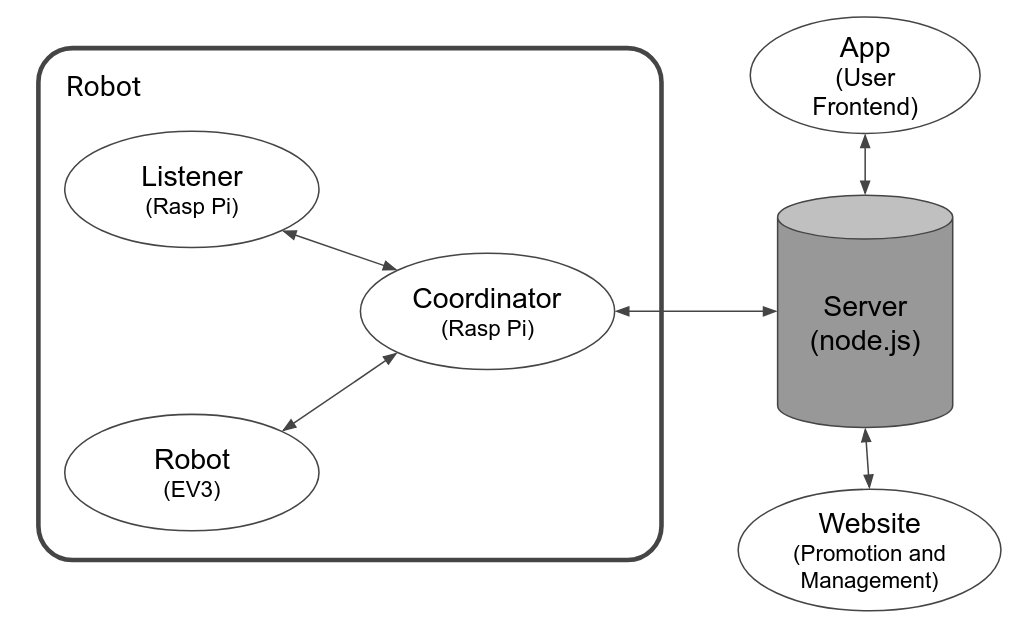
\includegraphics[width=0.9\textwidth]{sys.png}
    \caption{How the system communicates.}
    \label{fig: figure}
    \end{center}
\end{figure}

\section{Inventory}
Before setting up Bob please ensure that the following items are present in the supplied kit. You should have one of the following for the robot:
\begin{itemize}
    \item Bob robot
    \item Micro USB charger
    \item 10V DC transformer
    \item AA battery charger 
\end{itemize}

\section{Set Up}
Set up of the Bob system comprises of 3 primary sections:
\begin{enumerate}
    \item Setting up your account on our website.
    \item Setting up your warehouse.
    \item Setting up the robot. 
\end{enumerate}


\section{Server Set Up}
For development and testing purposes, the server can be set up locally in a closed-off network. Sysadmins of Bob can also deploy the server to cloud by following this section. \textbf{This is not needed for normal use. If you're a regular user (customer or merchant), skip this section.}

\subsection{Local Set Up}
For testing purposes only - if the internet is not available for your robot then you must set up the server and website yourself. Setting up the server will allow you to both locally host the webpage and the server to run the Bob app.
\begin{enumerate}
    \item Install node.js. OS specific instructions can be found at \underline{https://nodejs.org/en/download}. Node version 11.10.1 is known to work well.
    \item Clone the Bob git repository using the command below, this will pull all of the source code for the Bob system.
    \begin{lstlisting}[language=bash]
    $ git clone http://www.github.com/assis10t/bob.git
    \end{lstlisting}
    \item Navigate to the directory you just cloned and navigate into website. 
    \begin{lstlisting}[language=bash]
    $ cd bob/website
    \end{lstlisting}
    \item Once inside, execute the following to generate a local copy of the website. \begin{lstlisting}[language=bash]
    $ npm run generate
    \end{lstlisting}
    \begin{enumerate}[(a)]
        \item Note: For real deployment, you need to specify the URL where the server will be hosted before generating the website. Here’s the command for heroku deployment (replace the url with your heroku app's url): 
    \end{enumerate}
    \begin{lstlisting}[language=bash]
    $ BASE_URL=https://sdp-10-beta.herokuapp.com npm run generate
    \end{lstlisting}
    \item Once generated, copy the files in the generated folder into the /server/public.
    \begin{lstlisting}[language=bash]
    $ cp -r dist ../server/public
    \end{lstlisting}
    \item Install and run a mongodb instance in your machine, or use a cloud provider for mongodb. Instructions can be found at \underline{https://docs.mongodb.com/manual/installation/}.
    \begin{enumerate}[(a)]
        \item Note: You can skip this step if you’d like to use the built-in memory database for development purposes. 
    \end{enumerate}
    \item Go into the server directory, specify the mongodb connection url and start the server. Here’s the command for a local mongodb instance:
    \begin{lstlisting}[language=bash]
    $ cd ../server 
      MONGO=mongodb://localhost:27017/db npm start
    \end{lstlisting}
    \begin{enumerate}[(a)]
        \item Instead of a real mongodb instance, you may use the built-in in-memory database for development purposes. This will create a temporary mongodb instance that only lives in memory as long as the server is running.
    \end{enumerate}
    \begin{lstlisting}[language=bash]
    $ DB=memory npm start
    \end{lstlisting}
    \begin{enumerate}[(b)]
        \item For ease of development, a “development mode” is also available. This will run the server with an in-memory database and populate it with example data:
    \end{enumerate}
    \begin{lstlisting}[language=bash]
    $ npm run dev
    \end{lstlisting}
\end{enumerate}

\subsection{Deployment with Heroku}
\begin{enumerate}
    \item Set up a heroku account and create a new app. In the app’s settings, make sure it uses `heroku/nodejs` buildpack.
    \item Create a mongodb instance in the cloud. We’re using MondoDB Atlas, instructions for which can be found at \newline \underline{https://docs.atlas.mongodb.com/getting-started/}.
    \item In your heroku app’s settings, add a config var called MONGO, and set it to your cloud mongodb instance’s connection url.
    \item Follow the “Local Set Up” instructions up to and including step 5. At step 4, make sure you set the BASE\_URL to your heroku app’s url.
    \item Install the heroku CLI. Instructions for your platform can be found at \underline{https://devcenter.heroku.com/articles/heroku-cli}.
    \item Login to heroku using the following command:
    \begin{lstlisting}[language=bash]
    $ heroku login
    \end{lstlisting}
    \item Add your heroku app’s git URL as a remote to your local git repository as follows:
    \begin{lstlisting}[language=bash]
    $ git remote add heroku git@heroku.com:sdp-10-beta.git
    \end{lstlisting}
    \item Deploy the server using the following command:
    \begin{lstlisting}[language=bash]
    $ git push heroku `git subtree split --prefix server`:master --force
    \end{lstlisting}
\end{enumerate}

\section{Creating a Web Account}
Before you can define your warehouse layout and add items to your stock, you need to create an account on our website. The website is the control panel for merchants. From there you can set up multiple warehouses, describe their layouts, add and update stock, view and manage orders for a given warehouse, and authenticate customers when they come to collect an order using our QR code scanner.
\par You can create an account by navigating to http://sdp-10-beta.herokuapp.com/. Click on ‘Register’ and enter your credentials in the form. After you have chosen a valid username and password, click the ‘Sign-up’ button it you create your account.
\par To login, click on the ‘Login’ button at the top of the website then enter your username and password.
\begin{figure}[H]
    \begin{center}
    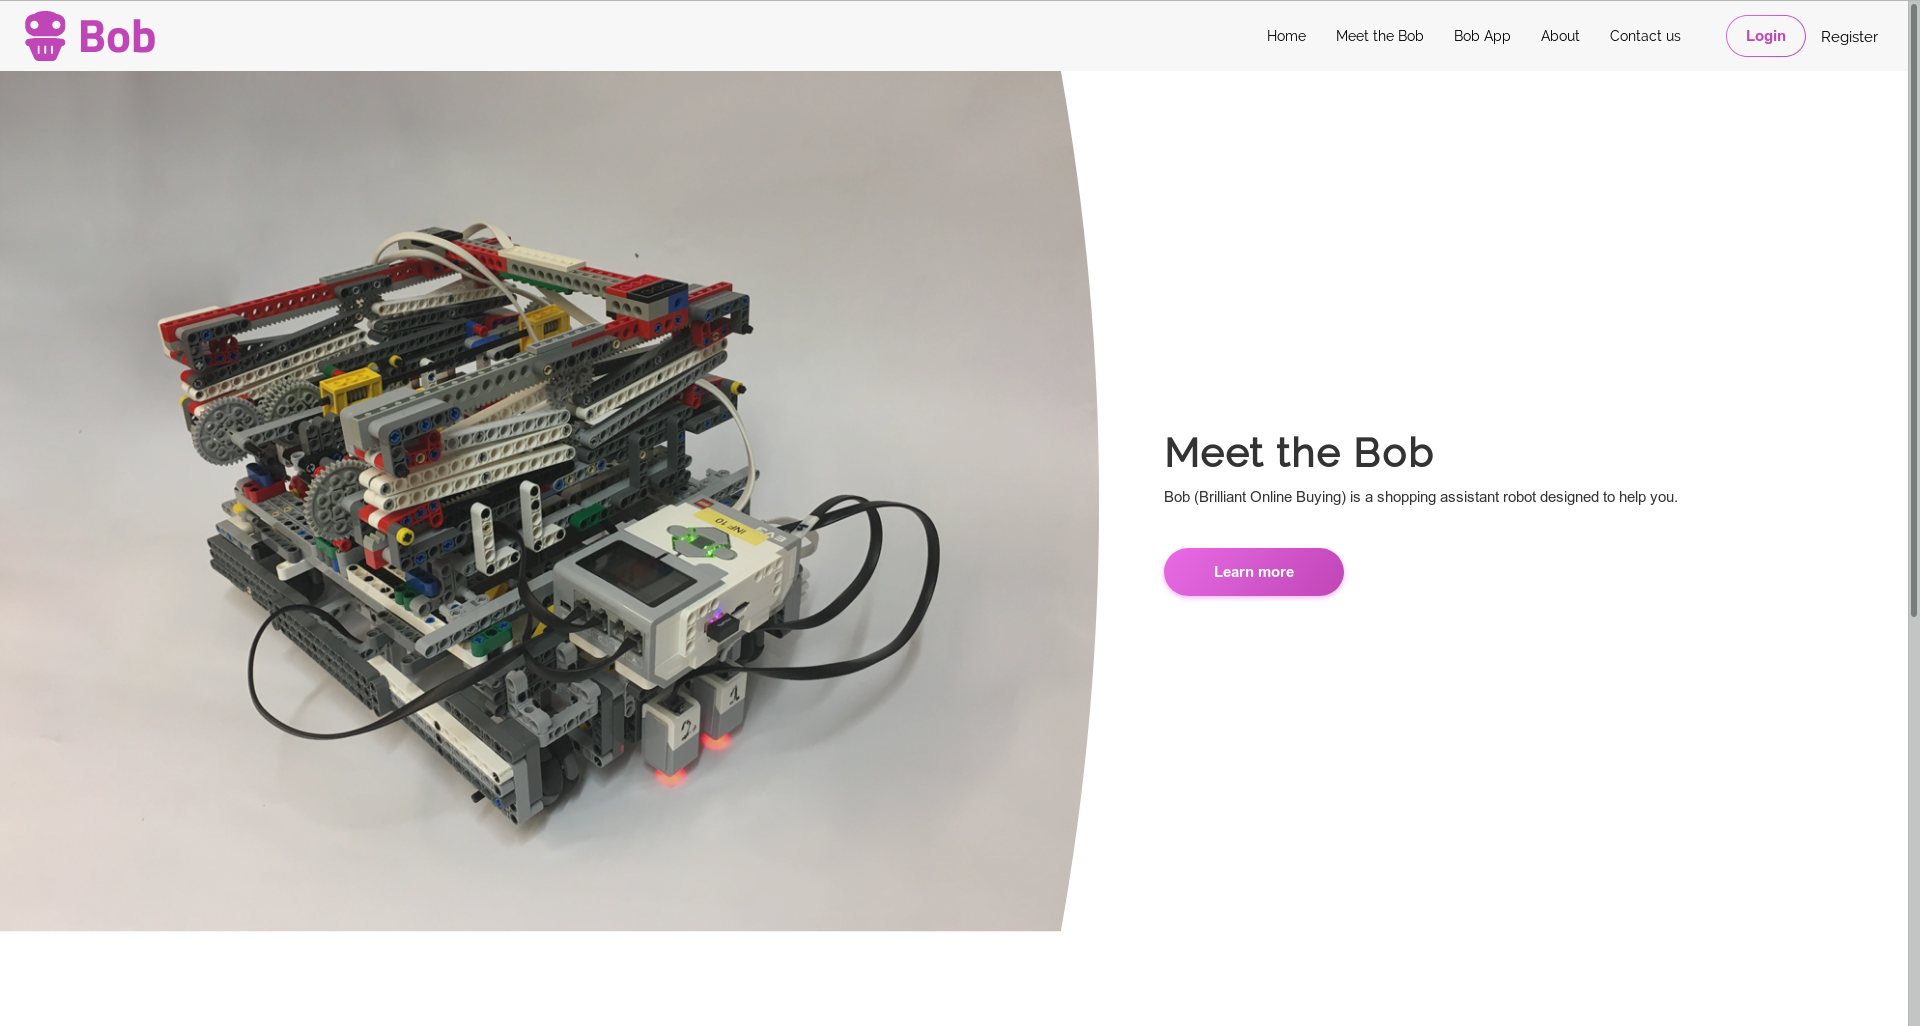
\includegraphics[width=1\textwidth]{website_homepage.png}
    \caption{Website homepage}
    \label{fig: figure}
    \end{center}
\end{figure}


\section{Creating a Warehouse}
\noindent\begin{minipage}{0.35\textwidth}
\begin{center}
    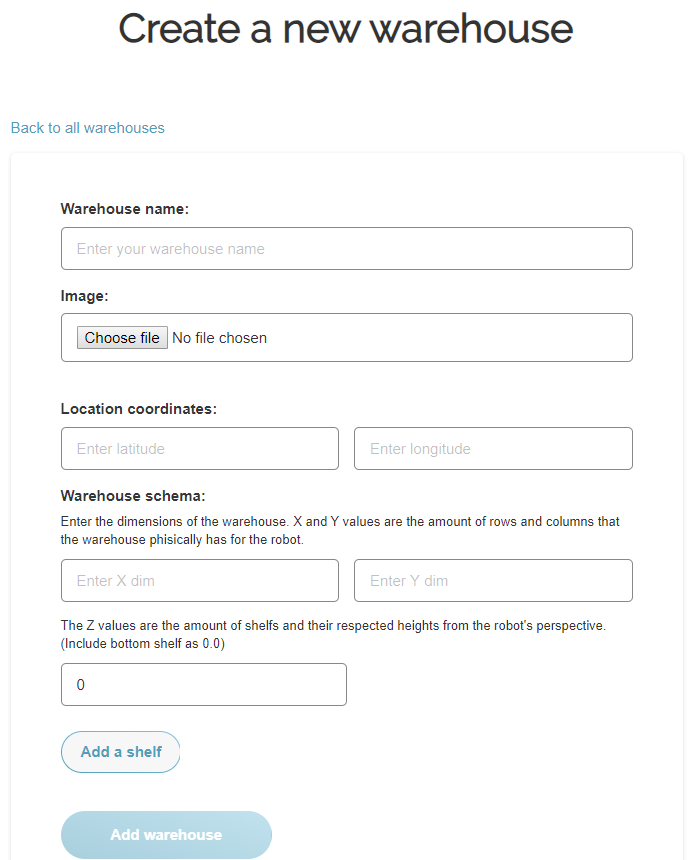
\includegraphics[width=\linewidth]{add-warehouse.PNG}
    \caption{Warehouse creation screen}
    \label{fig; figure}
\end{center}
\end{minipage}%
\hfill%
\begin{minipage}{0.65\textwidth}
Before you can get Bob to collect orders, the warehouse environment must be set up correctly. 
Bob uses lines on the ground to navigate around a warehouse. These can be made of either coloured tape or paint.
\begin{itemize}
    \item Black lines will create a path down the centre of aisles for the robot to follow. These lines do not need to be perfectly straight as Bob can maneuver along small bends in the path, however the robot was not designed to make sharp turns.  
    \item Green markings should be placed on the boundary between each shelf position down an aisle. These are used to keep track of the shelf Bob is currently at.
    \item Blue lines are placed in parallel at the end of the shelves. Bob will travel sideways in between the two lines to ensure he stays on track when moving between aisles.
    \item The floor should be white to increase the contrast between lines and the ground, and to prevent false colour readings from occurring. 
\end{itemize}

\end{minipage}

\subsection{Warehouse Dimensions}
For Bob to operate in your warehouse, you will need to set the warehouse up so that Bob can navigate around it. Please consult the following specifications and diagram provided to aid you in setting up your warehouse.

\subsubsection{Lines Dimensions}
\begin{itemize}
    \item Black lines are 2.5cm thick.
    \item Blue and green lines are 5cm thick.
\end{itemize}

\subsubsection{Space Requirements}
\begin{itemize}
    \item There must be a gap of at least 38 cm between pairs of blue lines or green lines. This is the distance between Bob’s front and back colour sensors.
    \item To prevent Bob crashing into shelves when moving sideways, allow for a gap of at least 2 cm between the outside of blue lines and shelves at Bob’s back side. Leave at least a further 12 cm on the front side to prevent Bob from crashing into anything there.
    \item The perpendicular distance from the centre of the black line to a shelf should be at least 23 cm.
    \item The shelves should be at least 25 cm deep however Bob will be unable to grab items further than 15 cm from the edge. The extra 10cm are needed for the claw of the grabber to extend outwards and scoop the item in.
    \item The bottom shelf should be 21.5 cm from the ground.
    \item The top shelf should be 45.5 cm from the ground.
    \item Bob grabs to his right so the shelves should be open on their left.
\end{itemize}
\  \\
The warehouse setup can be expanded very flexibly using the website; the only requirements are: 
\begin{enumerate}
    \item The warehouse is represented as a matrix.
    \item Each column in the matrix either has a black line running along it or a shelf (they can be interchanged as seen in the example layout).
    \item Each entry where Bob should pick an object up has to have a green line both in the front and back of it (to support backwards and forwards movement).
\end{enumerate}

\subsubsection{Example}
An example layout is depicted below. To start, Bob’s position should be in a side aisle between the two blue lines, e.g. in the lower right corner as shown.
\begin{figure}[H]
    \begin{center}
    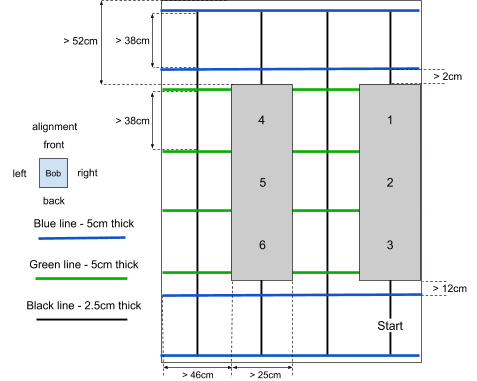
\includegraphics[width=0.6\textwidth]{layout.png}
    \caption{Layout in which Bob would function.}
    \label{fig: figure}
    \end{center}
\end{figure}
\begin{table}[H]
\begin{center}
\begin{tabular}{| p{0.4cm} | p{0.4cm} | p{0.4cm} | p{0.4cm} |}
\hline
\textbf{ } & \textbf{ } & \textbf{ } & \textbf{ } \\
\hline
  & 4 &   & 1 \\
\hline
  & 5 &   & 2 \\
\hline
  & 6 &   & 3 \\
\hline
  &   &   &   \\
\hline
\end{tabular}
\end{center}
\caption{Corresponding matrix representation.}
\end{table}
\begin{figure}[H]
    \begin{center}
    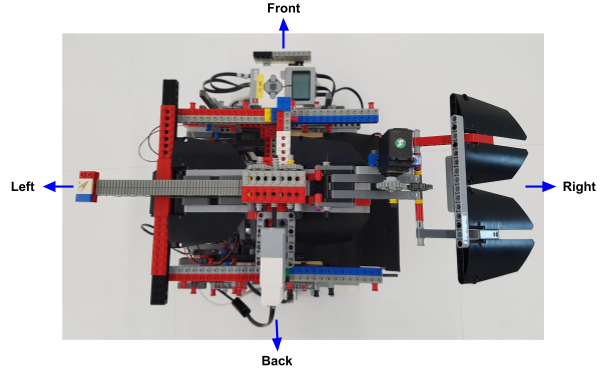
\includegraphics[width=0.9\textwidth]{top.png}
    \caption{Bob's sides labelled.}
    \label{fig: figure}
    \end{center}
\end{figure}

\subsection{Adding Warehouse On The Website}
After you have physically created the layout for your warehouse, you need to define these details online. Open the Bob website, access your account and navigate to ‘Warehouses’. This is the page that lists all of the warehouses that you have created and gives you options to view, edit and delete each one, and of course, to add a new warehouse.
\par After clicking on ‘Add a warehouse’ you are presented with a form. You are prompted to enter the name of the warehouse, add an image, enter the real coordinates (latitude and longitude) and define the warehouse schema. 
\par The first part of the warehouse layout is its dimensions. The X and Y values are the amount of rows and columns (respectively) that the warehouse has. When entering these values, keep in mind that the first row/column will be ‘0’. The second part is the vertical dimension - the amount of shelves. This Z value is different because you define each shelf separately by its physical height from the robot's perspective. (Include bottom shelf as 0.0)

\subsection{Add Stock}
It is now time to add stock to the  warehouse that you have just set up. As mentioned you can have multiple warehouses and each warehouse will have its own list of stock. 
\par After logging into your profile, navigate to the ‘Items’ page. If you have successfully created a warehouse, it will be automatically selected by the drop-down input in the page heading. Now you can begin uploading items by clicking on the blue  ‘Add items to this warehouse’ button.
\par You are given a form, which requires the name of the item and an image for the customer to see on their App. The position of the item inside the warehouse needs to be specified. The 3 inputs are for the X, Y and Z (shelf) values respectively. The quantity field requires an integer, and can be updated later on when restocking, the unit field is optional, and finally the price needs to be set in GBP. After putting in the necessary information, the ‘Add item’ button will activate and by pressing it, the item will be added.
\par Having uploaded multiple items, you can browse, edit and delete them using the ‘Items’ page, or inside the ‘View warehouse’ page.

\section{Connecting Bob To A Network}
Check the appendix to see where these are located on the Bob robot.\n
In order to collect orders, Bob must be connected to the Internet. 
\par Before setting up the Pi and EV3 make sure to have the details of the Wifi network (the SSID and password/key) you connect the robot to. If you are planning on using eduroam, obtain the set up details from your organisation. Both the EV3 and the Pi need to be on the same wifi network. Ensure this network has does not have client isolation
\footnote{\url{https://denon.custhelp.com/app/answers/detail/a_id/3746/~/wireless\%2C-ap-or-client-isolation}} 
enabled. Note in both cases, networks with browser based sign in processes will not work on either device due to their minimal GUI. 

\subsection{Connecting the Pi}
\begin{figure}[H]
    \begin{center}
    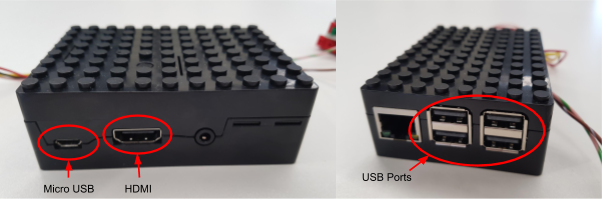
\includegraphics[width=0.7\textwidth]{pi-port.png}
    \caption{Ports to be connected.}
    \label{fig: figure}
    \end{center}
\end{figure}

\subsubsection{Set Up}
\begin{enumerate}
    \item To begin set up, plug the Pi into a monitor using a HDMI connection. Plug a keyboard into a USB port on the Pi as well. 
    \item Plug a micro USB cable which is connected to a power supply into the Pi’s micro USB  slot. You should see a flashing LED, indicating the  Pi is booting up.
    \item Once the Pi has booted, you will see a terminal prompt, execute the following steps on the Pi.
    \item Navigate to /etc/wpa\_spplicant (cd /etc/wpa\_supplicant), then open the “wpa\_supplicant.conf” file; this can be done using `sudo nano wpa\_supplicant.conf`. \textbf{It is important to run the with sudo access.}
    \item Once in the file, create a new network configuration, examples for regular wifi and eduroam can be seen in Figure whatever $<$screenshot of the file$>$
    \item Press Ctrl-O to save the file, then Ctrl-X to exit nano. 
\end{enumerate}
\  \\
Once the setup process is complete, take note of the IP address of the PI\footnote{\url{https://www.linuxtrainingacademy.com/determine-public-ip-address-command-line-curl/}} for connecting to the Pi to start bob. 

\subsection{Connecting the EV3}
Before beginning the EV3 set up ensure that the EV3 has battery power and that it has a USB Wifi Dongle plugged in, as shown below.
\begin{figure}[H]
    \center
    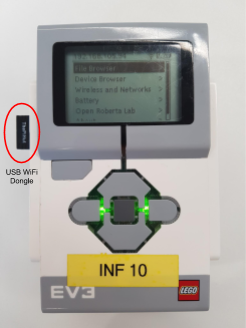
\includegraphics[width=0.2\textwidth]{ev3.png}
    \caption{Labelled EV3 Wi-Fi Dongle Port.}
    \label{fig: figure}
\end{figure}
\begin{enumerate}
    \item Check the Wifi dongle is connected to the EV3 brick in it’s USB slot. 
    \item Start the EV3 by pressing the centre button. Wait until you are presented with a menu on the listing ‘File Browser, Wireless and Networks’ etc. This step can take a few minutes so please be patient. 
    \item Once the EV3 has booted, navigate using the direction pad to the “Wireless and Networks” section and press the centre button proceed. Then navigate to the “Wifi settings”.
    \item Once in the Wifi settings, ensure that the “Powered” box is checked (filled with black). Move down and select “Start Scan”; you will see the option change to “Stop Scan”; Once the option has changed to back to “Start Scan”, navigate down to see a list of available networks.
    \item Select the network you wish to connect to; you will be presented with the settings screen for that network. Once on this network, select “Connect” and enter the password for the network. \item After this complete you will see “Status: Connected” as shown in \textbf{TODO: figure x.} Navigate to the “Network Connection” tab; select “Connect Automatically” to allow Bob to perform this automatically. 
    \item The EV3 is now connected to the network. 
\end{enumerate}

\section{Final Steps}
\subsection{Placing Bob in the Warehouse}
Place Bob in the start position indicated in the warehouse setup stage.

\subsection{Starting Bob}
\begin{enumerate}
    \item Using the IP address of the EV3, ssh into the EV3 using the following `ssh robot@$<$ip$>$` from a computer on the same network.
    \item Once you have an ssh session, run `./ev3\_listener.py`.
    \item In another terminal, use the IP address of the Pi to ssh into the Pi using the command `ssh student@ip`, from a machine on the same network.
    \item Once you have successfully “ssh”ed into the Pi, execute the command `./rasppi\_coordinator.py`, this will initiate Bob’s start up process. Bob will play 3 rising tones once ready to receive orders.
\end{enumerate}
\  \\
Bob is now set up and listening for orders, place an order at your store and make sure Bob can go and fetch it.

{\let\clearpage\relax \section{Day-to-Day Usage of Bob}}

\subsection{Update Stock}
You can easily update the stock on the website. After you have manually stocked the shelves log in to your merchant account and navigate to the items tab. You will see a list of all of the items currently for sale, scroll to the item you wish to update and click edit. You will be presented with the details of the items, increment the “quantity” as necessary then click update item. This will automatically make the new stock available to customers on the app, and the robot.
\begin{figure}[H]
    \begin{center}
    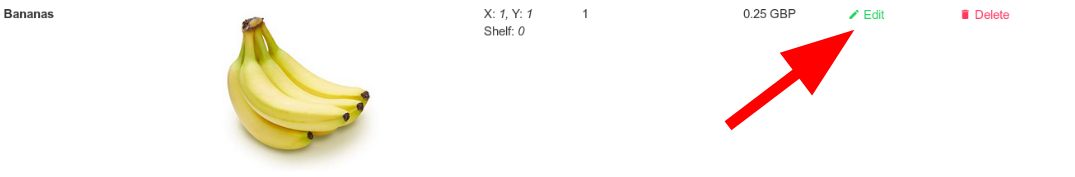
\includegraphics[width=1\textwidth]{update_stock.png}
    \caption{Edit warehouse}
    \label{fig: figure}
    \end{center}
\end{figure}

\subsection{Update Warehouse}
If you wish to update the warehouse schema, location or name, log on to your merchant account, navigate to the “Shops” tab. This will present you with a list  of all your shops; clicking edit will present you with a form to change the schema, location and name. Once done click “Update Warehouse”, this will automatically update the robot’s knowledge of the warehouse and the what the customers see on their app. 
\begin{figure}[H]
    \begin{center}
    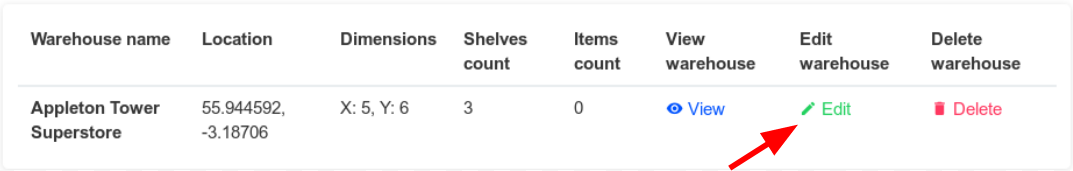
\includegraphics[width=1\textwidth]{update_warehouse.png}
    \caption{Item in stock list}
    \label{fig: figure}
    \end{center}
\end{figure}

\subsection{Charging}
There are three separate power sources on Bob:
\begin{enumerate}
    \item EV3 Rechargeable DC Battery.
    \item 5000mAh Powerbank.
    \item 8 AA rechargeable batteries in a single 8-way battery holder.
\end{enumerate}
The location of these items can be seen in the appendix.
\newline
Charging the EV3 Battery:
\newline
The system will check the battery level of the EV3 in between orders and provide a warning when power is low. 
\newline
To charge the EV3, plug the 10V DC transformer into the charger slot at the base of the EV3 brick (circled below), you do not need to remove the EV3 from the robot in order to charge it.  
\begin{figure}[H]
    \begin{center}
    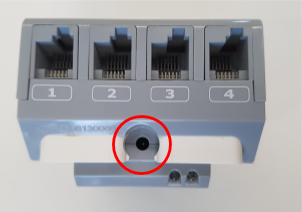
\includegraphics[width=0.5\textwidth]{ev3-charge.png}
    \caption{EV3 Charging Port.}
    \label{fig: figure}
    \end{center}
\end{figure}
\begin{figure}[H]
    \begin{center}
    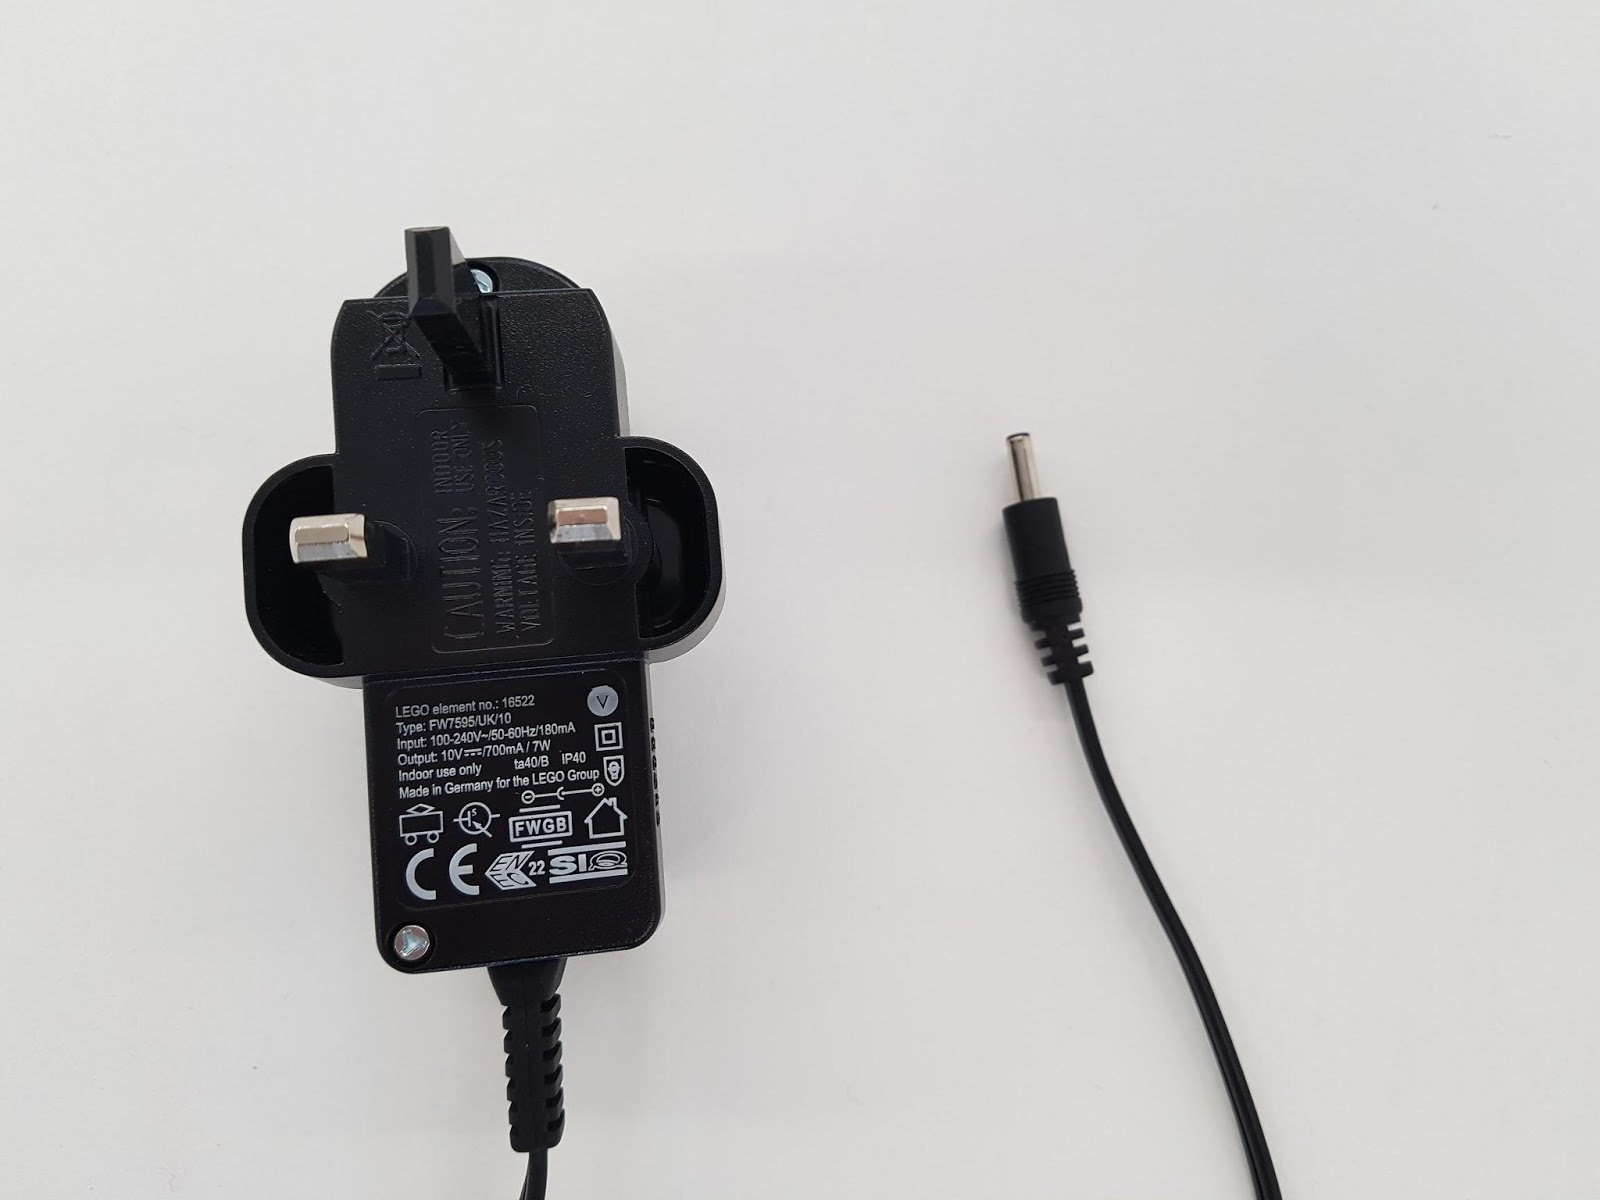
\includegraphics[width=0.5\textwidth]{ev3-adapter.jpg}
    \caption{10V DC transformer.}
    \label{fig: figure}
    \end{center}
\end{figure}
\  \\
Charging the powerbank:
\newline
The powerbank will show its power level via 4 blue lights on its front. When the battery is low, unplug the two USB leads connected to the powerbank and plug in the micro USB charger. When the powerbank is fully charged, unplug it from the charger and reconnect the USB leads into their matching ports. Return the powerbank to its slot on the robot.
Important: Do not charge the powerbank while it is still connected to the robot.
\begin{figure}[H]
    \begin{center}
    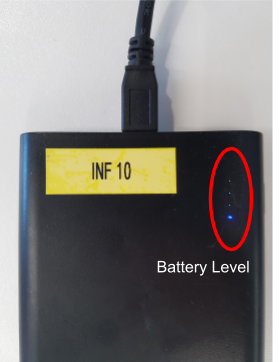
\includegraphics[width=0.5\textwidth]{power.png}
    \caption{Charging powerbank.}
    \label{fig: figure}
    \end{center}
\end{figure}
\begin{figure}[H]
    \begin{center}
    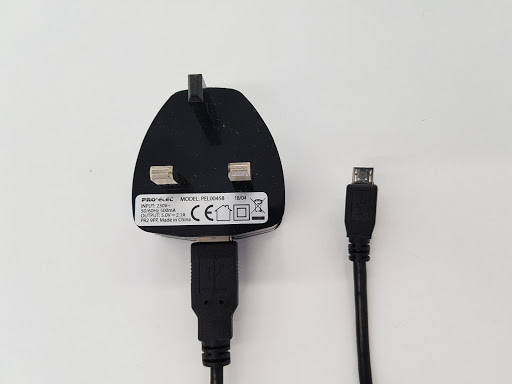
\includegraphics[width=0.5\textwidth]{usb.jpg}
    \caption{Micro USB Charger.}
    \label{fig: figure}
    \end{center}
\end{figure}
\begin{figure}[H]
    \begin{center}
    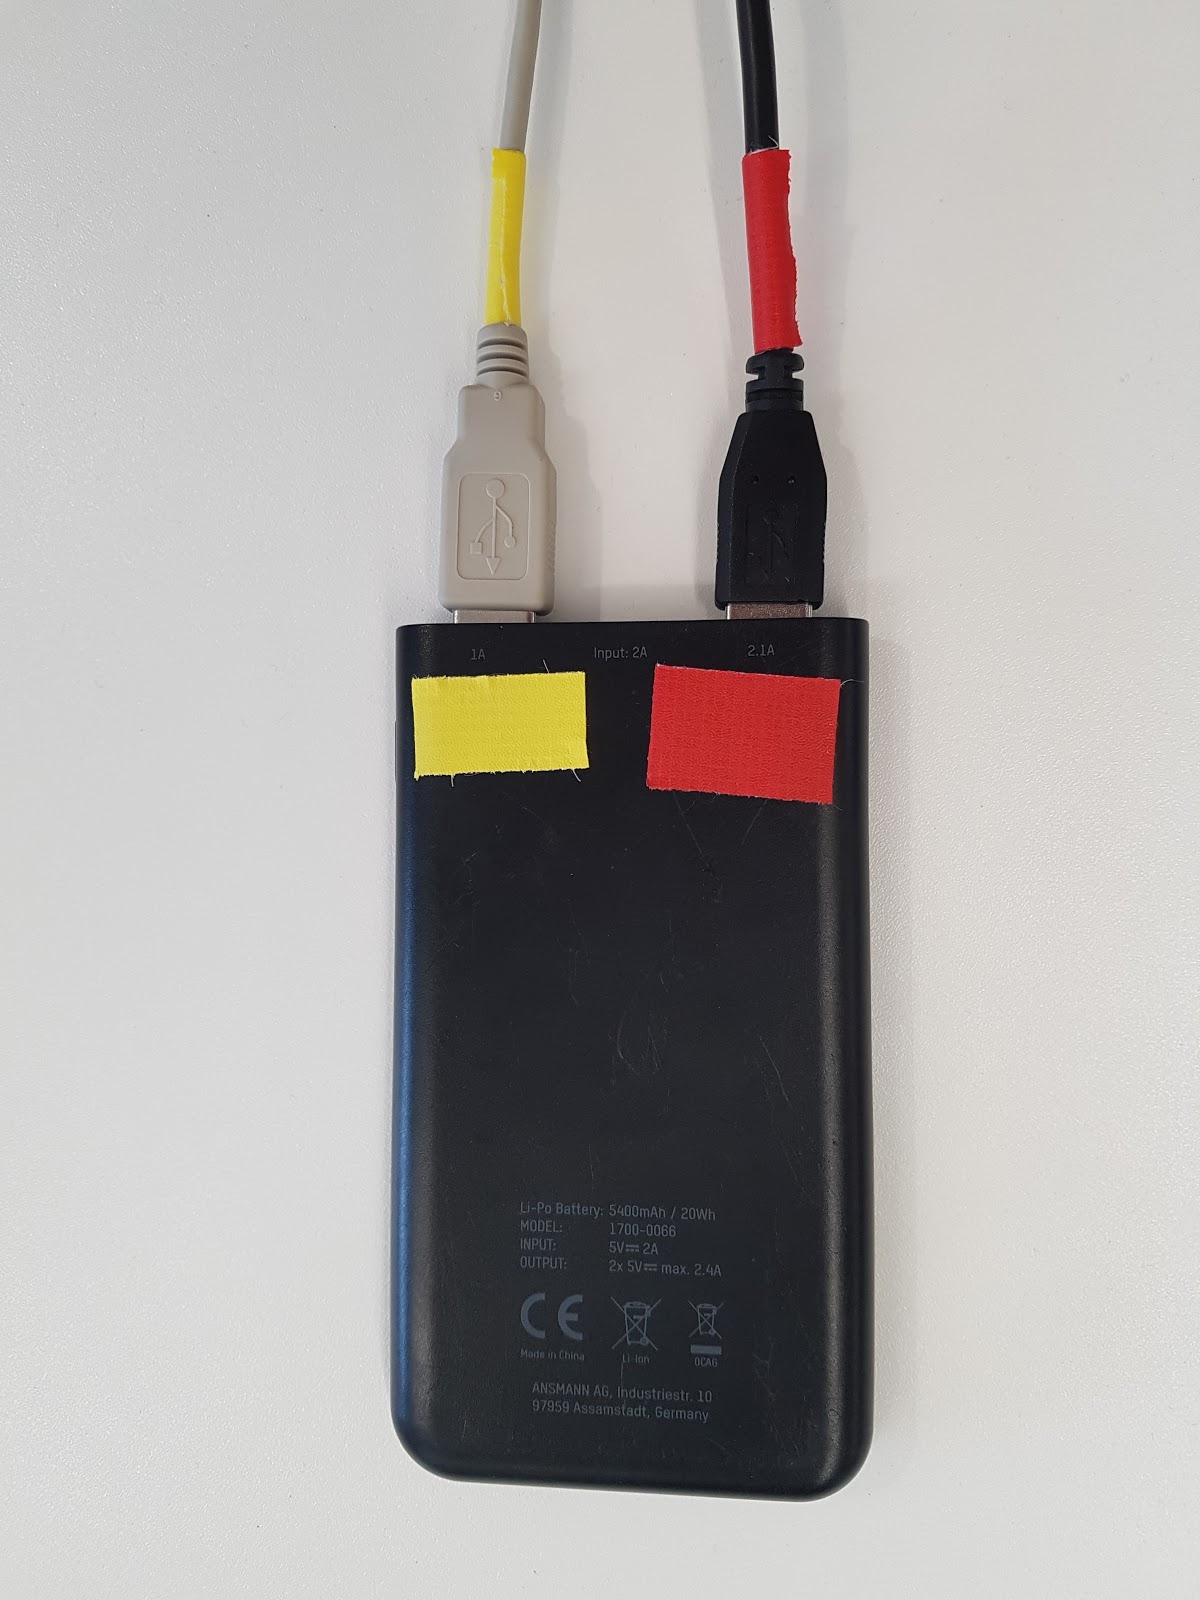
\includegraphics[width=0.5\textwidth]{connect-pwrbnk.jpg}
    \caption{Reconnecting powerbank to robot.}
    \label{fig: figure}
    \end{center}
\end{figure}
\  \\
Charging the AA batteries:
\newline
The AA batteries should be charged once a day. To charge the batteries, disconnect the battery holder from the robot and remove the batteries from it. The batteries can be recharged in the battery charger. When the batteries are fully charged, place them back into the battery holder and reattach it to the robot.
\begin{figure}[H]
    \begin{center}
    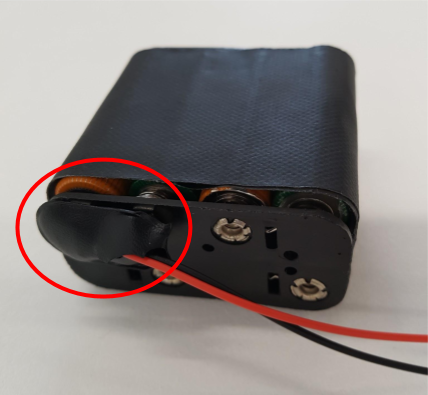
\includegraphics[width=0.5\textwidth]{battery-detach.png}
    \caption{Detach the battery holder before removing batteries.}
    \label{fig: figure}
    \end{center}
\end{figure}
\begin{figure}[H]
    \begin{center}
    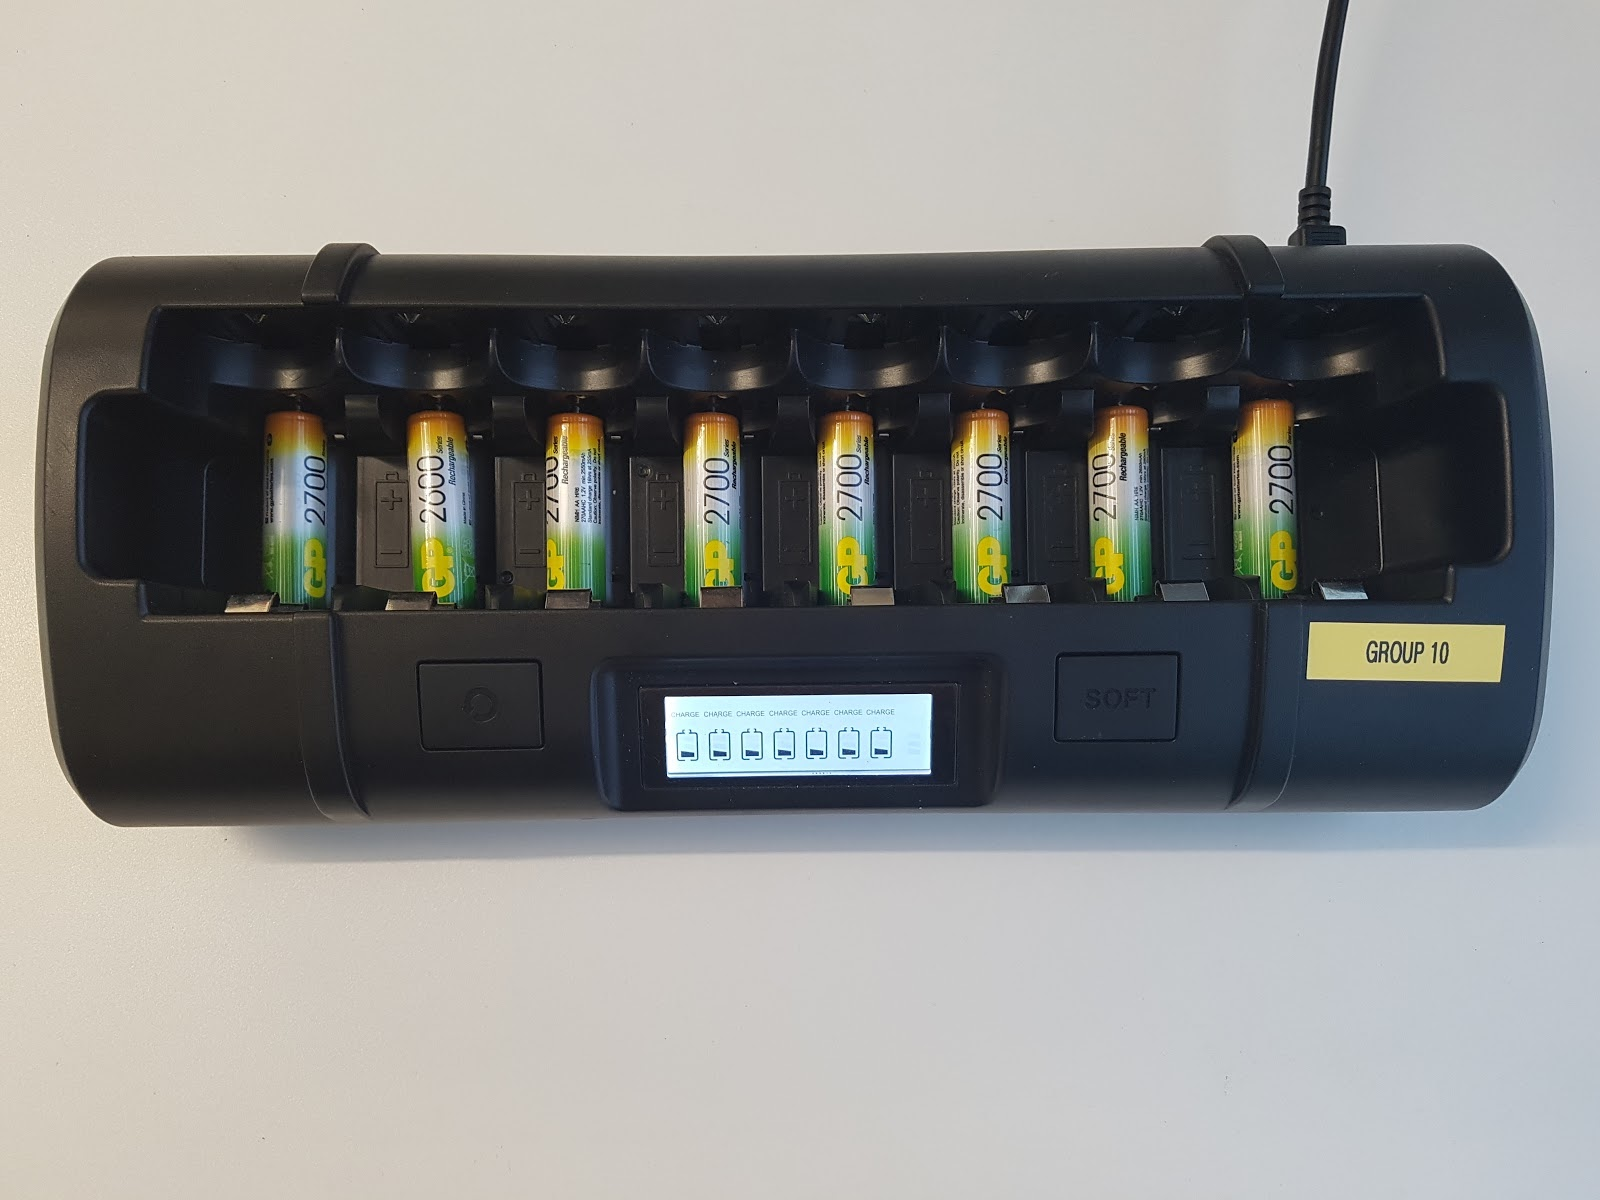
\includegraphics[width=0.5\textwidth]{battery-recharge.jpg}
    \caption{Battery charger displaying level of charge.}
    \label{fig: figure}
    \end{center}
\end{figure}

{\let\clearpage\relax \section{App}}
This app is aimed at the customer of the shop

\subsection{Install App}
\begin{enumerate}
    \item Make sure your Android device or emulator uses Android 6.0 or above. 
    \item Enable installation of apps from unknown sources by navigating to Settings > Security > Unknown Sources. Note that the location of this setting may vary between Android devices.
    \item Navigate to https://github.com/Assis10t/bob/releases and and download the latest release of “app.apk”. (If using a development version of the app this file will be “app-debug.apk”) 
\end{enumerate}
\subsection{Using the App}
\begin{table}[H]
  \centering
  \begin{tabular}{ | m{5.5cm} | m{5.5cm} | m{5.5cm} | }
    \hline
    \begin{minipage}{.31\textwidth}
      
\includegraphics[width=\linewidth, height=90mm]{one.jpg}
    \end{minipage}
    1. At the beginning, the app will try to connect to the server automatically. If this happens, skip to step 4. Otherwise, tap the menu on the top right.
    &
    \begin{minipage}{.31\textwidth}
      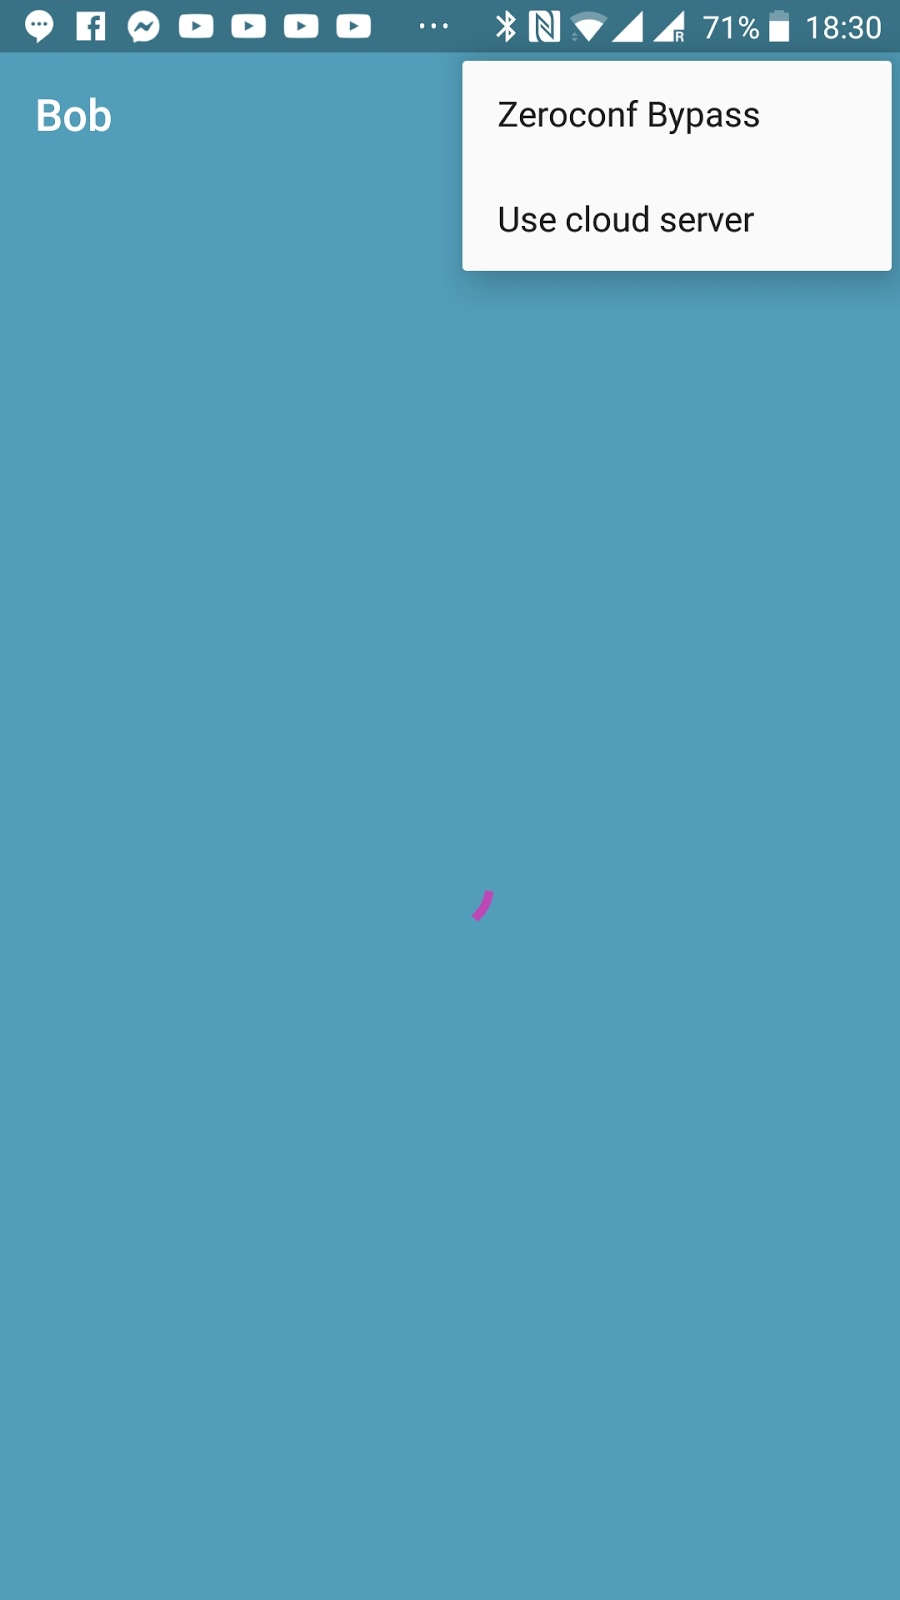
\includegraphics[width=\linewidth, height=90mm]{two.jpg}
    \end{minipage}
    2. To connect to the cloud server hosted on heroku, select “Use cloud server” and skip to step 4. Otherwise, select “Zeroconf Bypass”.
    & 
    \begin{minipage}{.31\textwidth}
      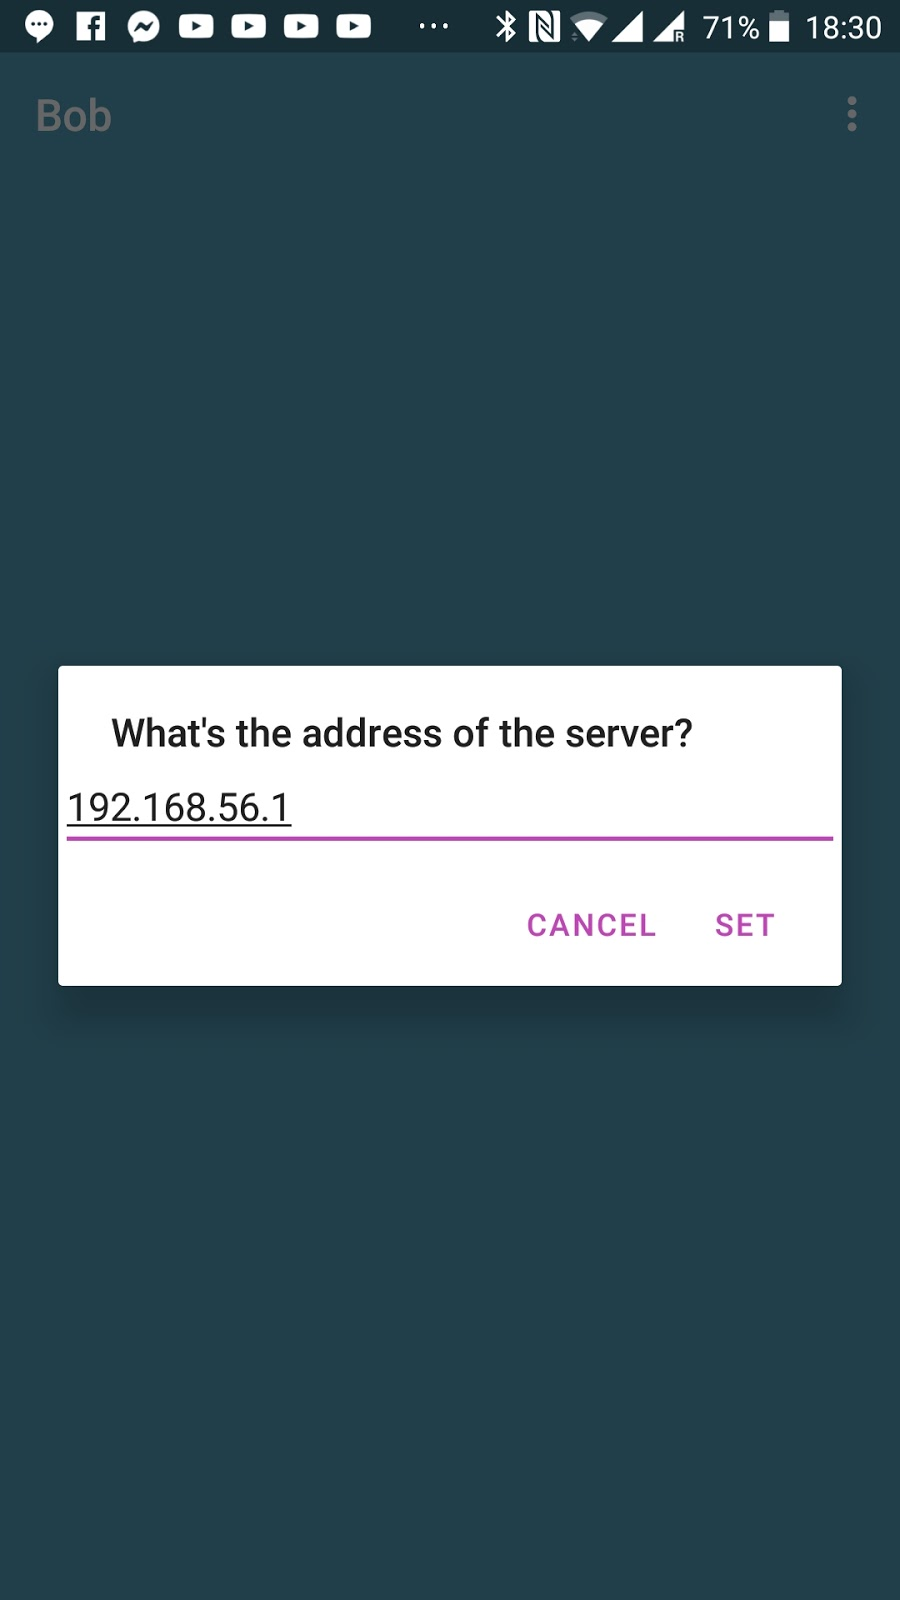
\includegraphics[width=\linewidth, height=90mm]{three.jpg}
    \end{minipage}
    3. Type the IP address of the local server, or the URL of the custom cloud server.
    \\ \hline
    \begin{minipage}{.31\textwidth}
      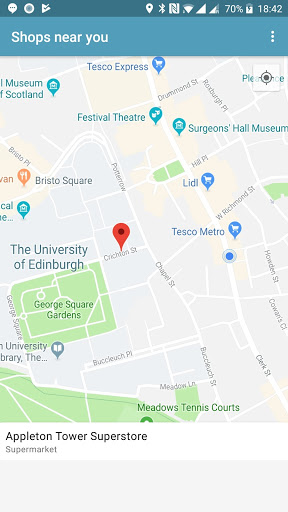
\includegraphics[width=\linewidth, height=90mm]{four.jpg}
    \end{minipage}
    4. You can see a list of shops you can order from near you. If you’re logged in, tap one of the shops and skip to step 7. Otherwise, tap the menu on the top right.
    &
    \begin{minipage}{.31\textwidth}
      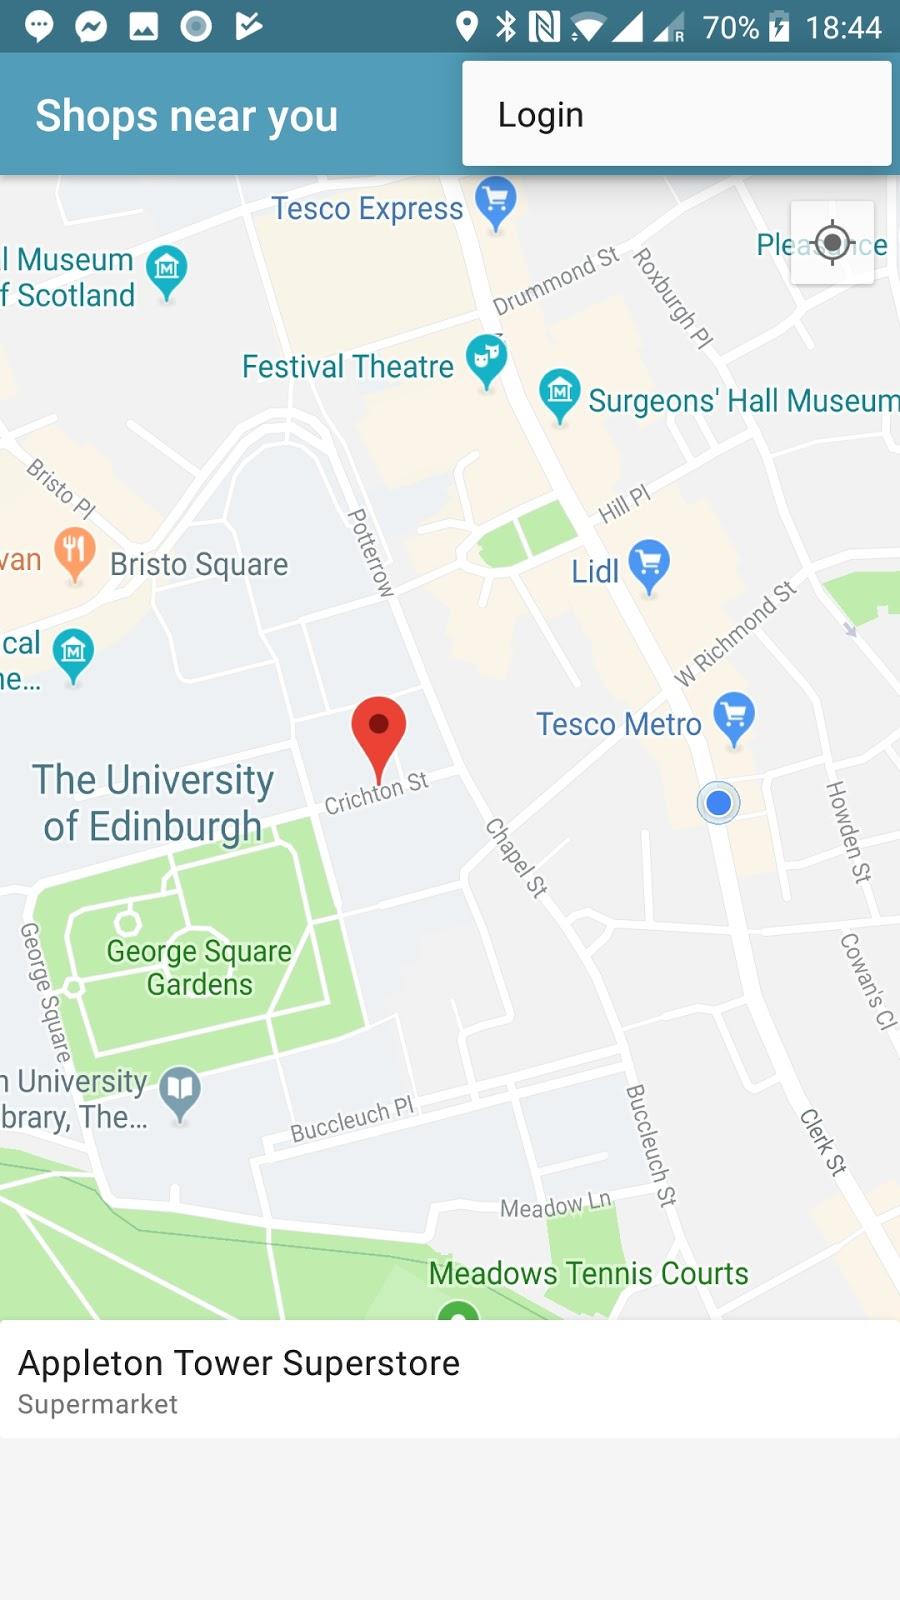
\includegraphics[width=\linewidth, height=90mm]{five.jpg}
    \end{minipage}
    5. If you see a “Login” button, tap it. If you see a welcome message, you are already logged in, so go back to step 4.
    & 
    \begin{minipage}{.31\textwidth}
      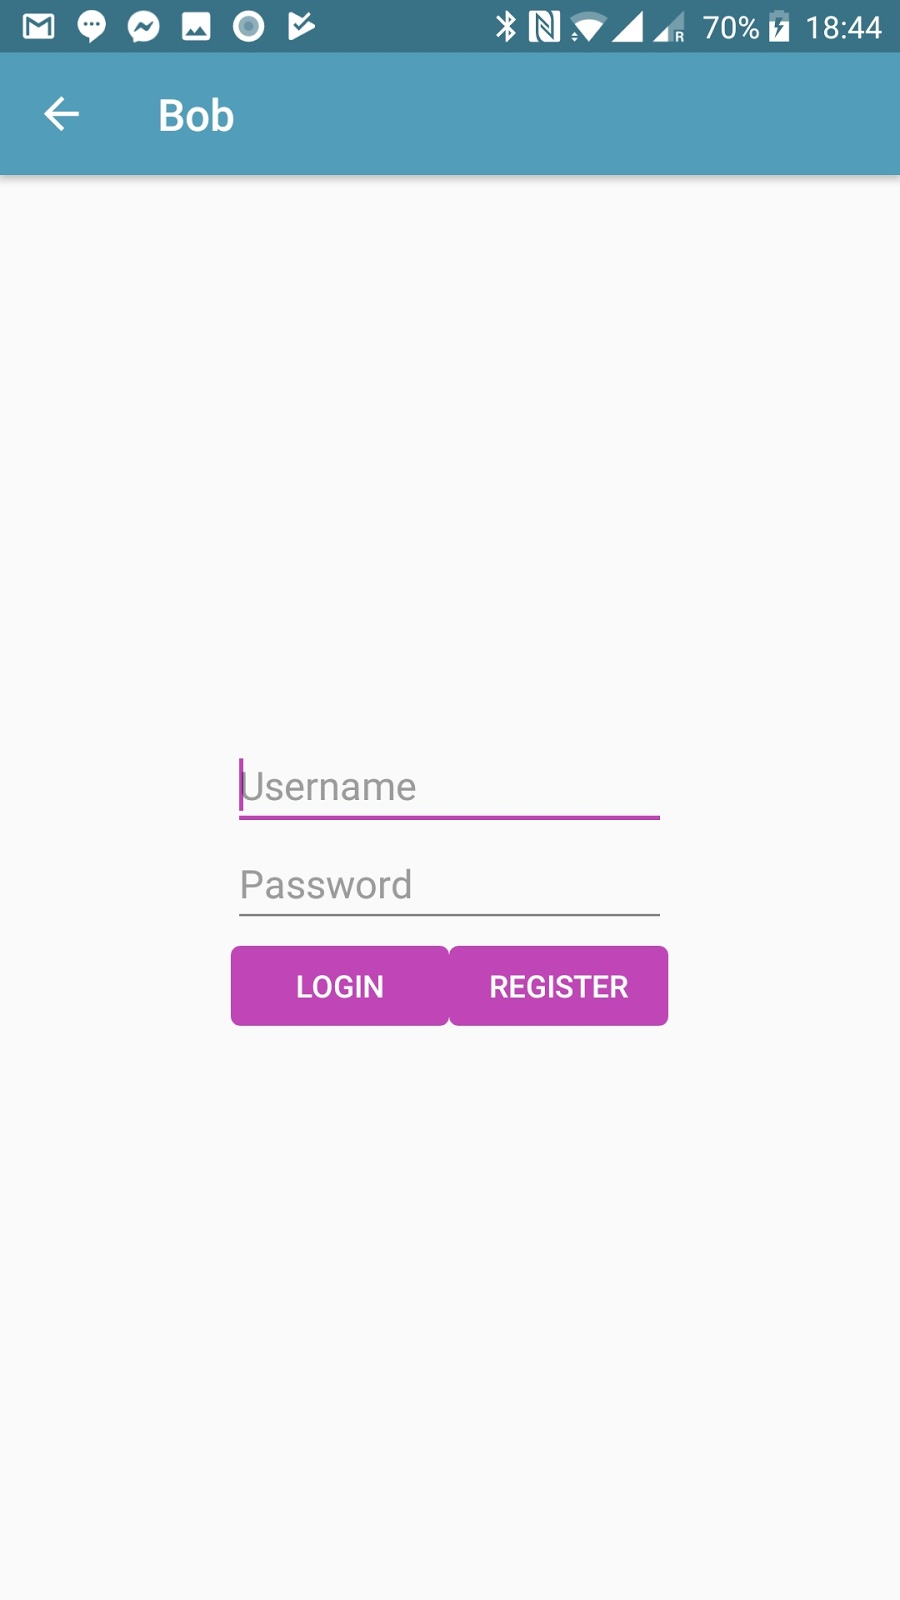
\includegraphics[width=\linewidth, height=90mm]{six.jpg}
    \end{minipage}
    6. Enter your e-mail address and password, and tap “Register” to create an account, or “Login” if you have an account already.
    \\ \hline
  \end{tabular}
  \caption{App for customer part 1.}\label{tbl:myLboro}
\end{table}

\begin{table}[H]
  \centering
  \begin{tabular}{ | m{5.5cm} | m{5.5cm} | m{5.5cm} | }
    \hline
    \begin{minipage}{.31\textwidth}
      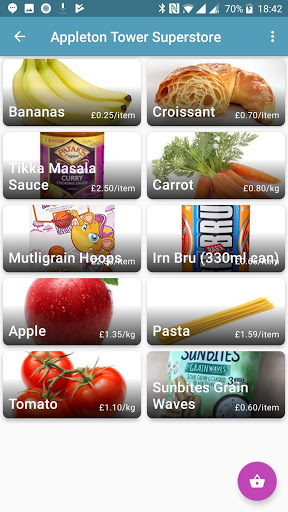
\includegraphics[width=\linewidth, height=90mm]{seven.jpg}
    \end{minipage}
    7. You can see a list of items in the shop you selected. To add one to your shopping cart, tap it and go to step 8. To complete your order, tap the shopping cart icon on the bottom right and go to step 9.
    &
    \begin{minipage}{.31\textwidth}
      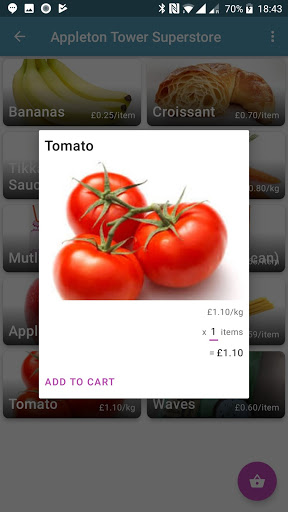
\includegraphics[width=\linewidth, height=90mm]{eight.jpg}
    \end{minipage}
    8. You can see the details on this item and how much it will cost. You may edit the amount you’d like by tapping the number in “x 1 items”. Once you’re ready, tap “Add to Cart” and go back to step 7.
    & 
    \begin{minipage}{.31\textwidth}
      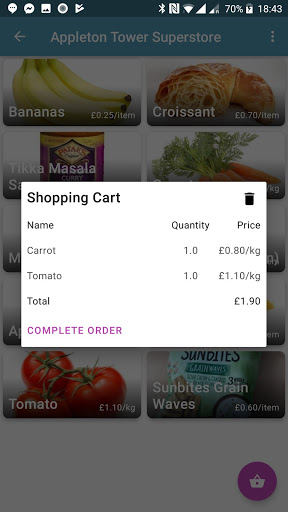
\includegraphics[width=\linewidth, height=90mm]{nine.jpg}
    \end{minipage}
    9. You may see every item you added to your shopping cart, and the total cost of all of the items. To clear your shopping cart, tap the trash can icon on the top right. To complete your order, tap the “Complete Order” button.
    \\ \hline
    \begin{minipage}{.31\textwidth}
      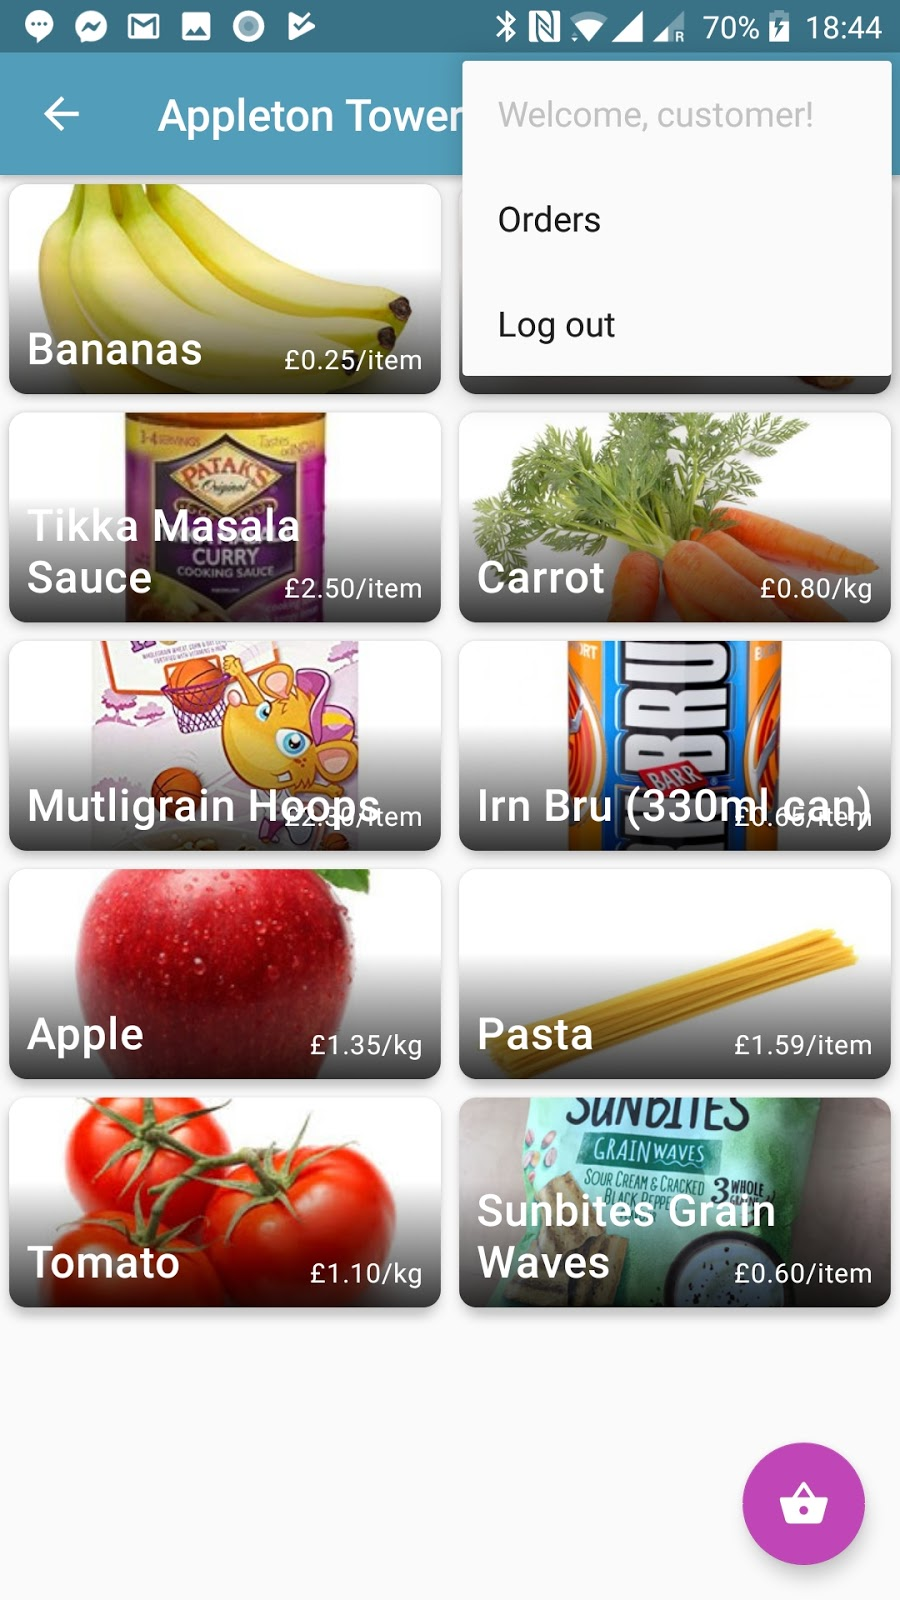
\includegraphics[width=\linewidth, height=90mm]{ten.jpg}
    \end{minipage}
    10. To view the status of your order or to collect your order, tap the menu on the top right, then tap “Orders”.
    &
    \begin{minipage}{.31\textwidth}
      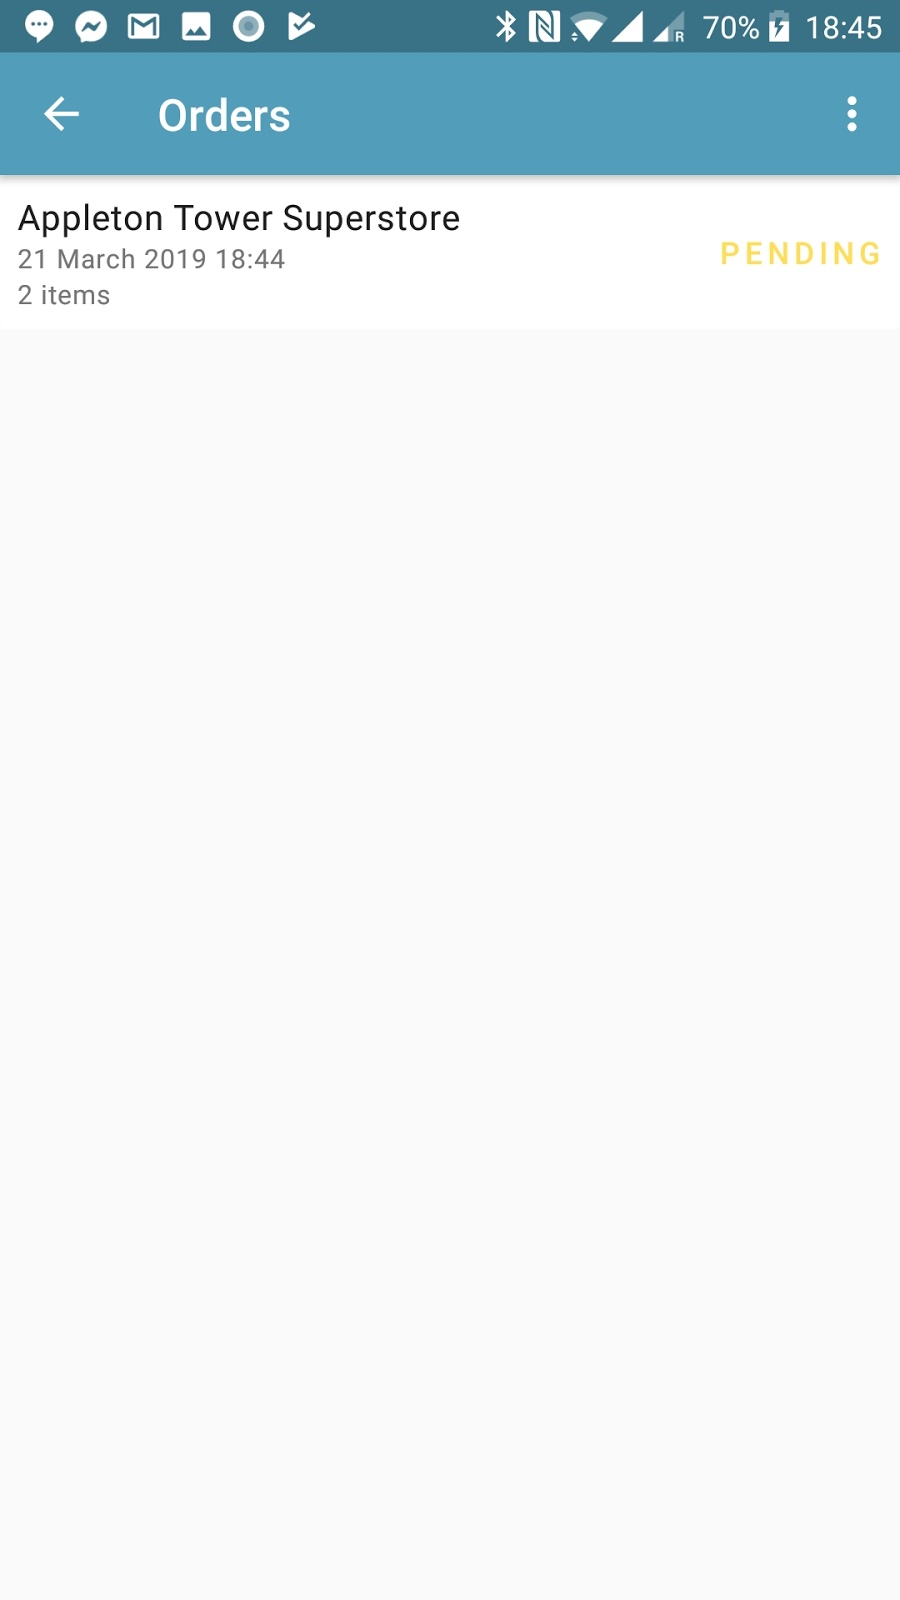
\includegraphics[width=\linewidth, height=90mm]{eleven.jpg}
    \end{minipage}
    11. You can see the list of all orders you made in the past, and their status. Tap an order to view the details, or to collect.
    & 
    \begin{minipage}{.31\textwidth}
      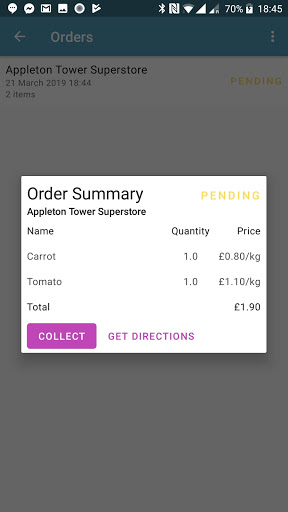
\includegraphics[width=\linewidth, height=90mm]{twelve.jpg}
    \end{minipage}
    12. You can see the details and status of your order. If the order is ready, tap “Collect” to collect it, or tap “Get Directions” to navigate to the store.
    \\ \hline
  \end{tabular}
  \caption{App for customer part 2.}\label{tbl:myLboro}
\end{table}

\begin{table}[H]
  \centering
  \begin{tabular}{ | m{5.5cm} | m{5.5cm} | m{5.5cm} | }
    \hline
    \begin{minipage}{.31\textwidth}
      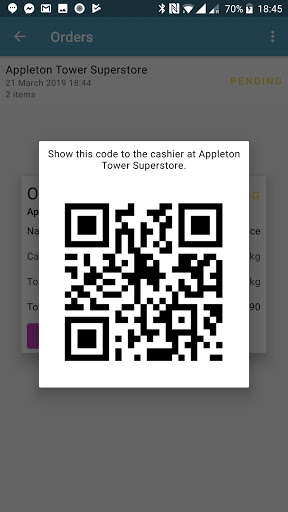
\includegraphics[width=\linewidth, height=90mm]{thirteen.jpg}
    \end{minipage}
    13. Show the store clerk this QR code in order to collect your order.
    &
    \begin{minipage}{.31\textwidth}
      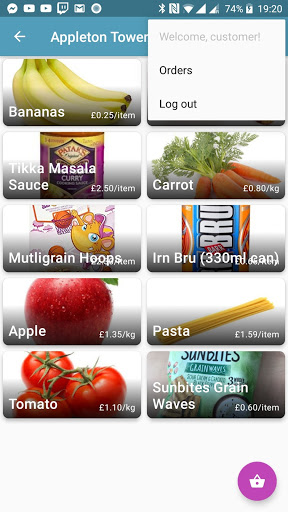
\includegraphics[width=\linewidth, height=90mm]{fourteen.jpg}
    \end{minipage}
    14. To log out at any point, tap the menu on the top right, and tap “Log out”.
    &
    
    \\ \hline
  \end{tabular}
  \caption{App for customer part 3.}\label{tbl:myLboro}
\end{table}

{\let\clearpage\relax \section{Troubleshooting}}
\begin{table}[H]
  \centering
  \begin{tabular}{ | m{0.4cm} | m{3.5cm} | m{3.5cm} | m{10cm} | }
    \hline
    ID & Problem & Likely Cause & Solution
    \\ \hline
    1 & Password Forgotten. & User forgotten password. & If you have forgotten your password, press the “Forgotten Password” button on the login page for either the App or website, this will then prompt you to enter your email address, and you will be sent a link to change your password. 
    \\ \hline
    2 & An order placed by a customer has not been collected. & Customer has not collected an order. & If an order has not been collected at the end of the day, it will be marked as such and the stock can be re-added to the warehouse. All you need to do is place the unclaimed stock back on the shelves.
    \\ \hline
    3 & BOB fails to return. & Bob is stuck or lost & If BOB fails to return with an order, disable him as described in section TODO, then you can go into the warehouse and find him. If he has not returned, his navigation has failed and he has gotten stuck. For troubleshooting navigation failure, see problem \#14.
    \\ \hline
    4 &  & The battery has died. & The robot may be unable to return if its battery level is too low. See the charging section to learn how to recharge batteries then place the robot back in the start position.
    \\ \hline
    5 &  & EV3 has crashed. & If there is an error showing on the EV3, it has crashed. See problem \#8. 
    \\ \hline
    6 & BOB returns with no item. & Stock incorrect. & If BOB returns, but does not have an item, then the first thing to do is check the stock in the store itself. And then update the stock on the website to match this as described in section \textbf{TODO.}
    \\ \hline
    7 &  & Unable to grab. & If the stock was in fact correct, check that the grabber is not being obstructed.
    \\ \hline
    8 &  & Navigation issue. & If the stock was correct, and the grabber is not obscured, then this may be a navigation issue, see problem \#14.
    \\ \hline
    9 & BOB returns with an incorrect item. & Items placed wrong. & If BOB returns with the incorrect item check that we website correctly corresponds with where the items are located.
    \\ \hline
    10 &  & Navigation issue. & If the website is correct, then this is likely a navigation issue, see problem \#14.
    \\ \hline
    11 & No Connection. & Robot is not connected to the network. & Check the network settings then try to ping the EV3 and Raspberry Pi using `ping $<$ip$>$` to check the connection.
    \\ \hline
    12 & BOB fails to follow the paths between shelves. & Navigation Issue. & If you can see that BOB is failing to follow the paths between shelves, this is a navigation failure, refer to problem \#14.
    \\ \hline 
    13 & The EV3 has crashed. & EV3 encountered error. & If you find that the EV3 has an error message on it, it has crashed. Check all motors and sensors are connected to the correct ports (appendix), the restart ev3listener.py.
    \\ \hline
    14 & Navigation Failure. & Colour sensors obstructed. & Check colour sensors (diagram TODO are not obstructed) and if there is any obstruction over the sensor, remove it so the sensor has clear sight on the floor.
    \\ \hline
    15 &  & Obstacle. & Check for obstacles on any part of the path, such as fallen items or other debris.
    \\ \hline
    16 &  & Lines laid incorrect. & Check lines are laid as described in section TODO. If they are laid incorrectly, make amendments as appropriate to correct this.
    \\ \hline
    17 &  & Dirty floor. & Bob relies on clear contrasting colours, dirty flooring may disrupt this, so try to keep the floor as clean and white as possible.
    \\ \hline
    18 &  & Other. & Relay the lines on the floor as described in section TODO, removing the old ones.
    \\ \hline
    19 & BOB does not start. & No network connection. & \textbf{TODO}
    \\ \hline
    20 &  & Incorrect wiring. & Check all motors and sensors are connected to the correct ports, as outlined in section TODO then restart BOB as outlined in section TODO.
    \\ \hline
  \end{tabular}
  \caption{Troubleshooting Table.}\label{tbl:myLboro}
\end{table}

\appendix
\begin{figure}[H]
    \begin{center}
    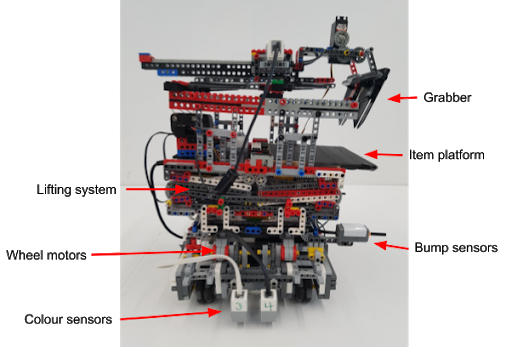
\includegraphics[width=0.6\textwidth]{bob_diagram.png}
    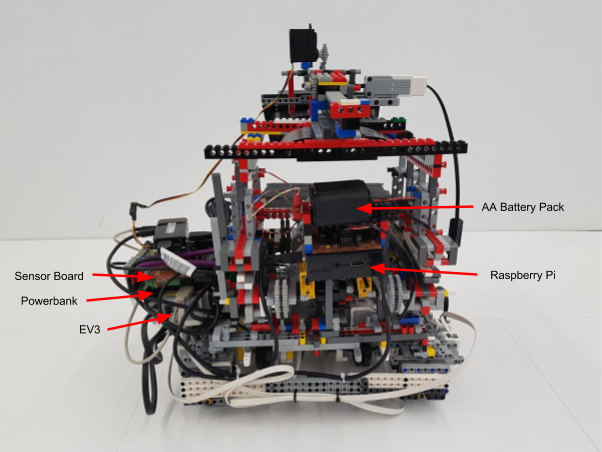
\includegraphics[width=0.6\textwidth]{bob_diagram2.png}
    \caption{Labelled BOB.}
    \label{fig: figure}
    \end{center}
\end{figure}
\begin{figure}[H]
    \begin{center}
    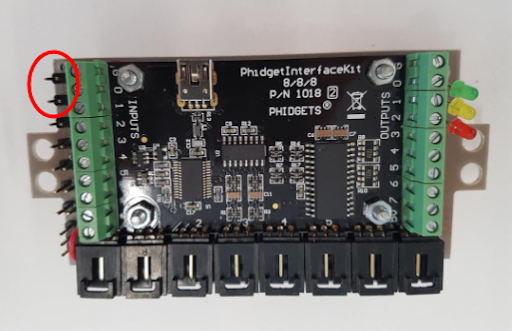
\includegraphics[width=0.5\textwidth]{bumper.png}
    \caption{If bump sensor wires become detached, put in ports 0 and 1 circled above.}
    \label{fig: figure}
    \end{center}
\end{figure}
\begin{figure}[H]
    \begin{center}
    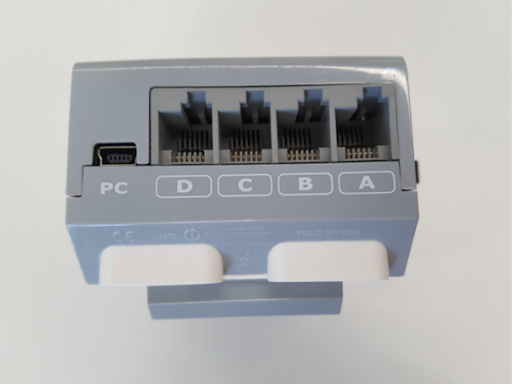
\includegraphics[width=0.5\textwidth]{wheel.png}
    \caption{If the wheel motor wires become detached, connect the wires to the port that matches the letter on the motor.}
    \label{fig: figure}
    \end{center}
\end{figure}
\begin{figure}[H]
    \begin{center}
    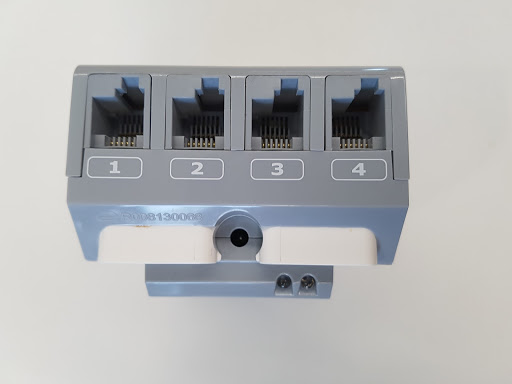
\includegraphics[width=0.5\textwidth]{colour.jpg}
    \caption{If colour sensor wires become detached, connect the wires to the port that matches the number on the sensor.}
    \label{fig: figure}
    \end{center}
\end{figure}

\end{document}
